%%%%%%%%%%%%%%%%%%%%%%%%%%%%%%%%%%%%%%%%%%%%%%%%%%%%%%%%%%%%%%%%%%%%%%%%%%%%%%%%
%2345678901234567890123456789012345678901234567890123456789012345678901234567890
%        1         2         3         4         5         6         7         8

%\documentclass[letterpaper, 10 pt, conference]{ieeeconf}  % Comment this line out
                                                          % if you need a4paper
\documentclass[a4paper, 10pt, conference]{ieeeconf}      % Use this line for a4
                                                          % paper

\IEEEoverridecommandlockouts                              % This command is only
                                                          % needed if you want to
                                                          % use the \thanks command
\overrideIEEEmargins
% See the \addtolength command later in the file to balance the column lengths
% on the last page of the document


\usepackage{comment}
% The following packages can be found on http:\\www.ctan.org
\usepackage{graphicx} % for pdf, bitmapped graphics files
%\usepackage{epsfig} % for postscript graphics files
%\usepackage{mathptmx} % assumes new font selection scheme installed
%\usepackage{times} % assumes new font selection scheme installed
%\usepackage{amsmath} % assumes amsmath package installed
%\usepackage{amssymb}  % assumes amsmath package installed

%-Para bash and c++
\usepackage{listings}

\usepackage{xcolor}
\begin{comment}

\definecolor{codegreen}{rgb}{0,0.6,0}
\definecolor{codegray}{rgb}{0.5,0.5,0.5}
\definecolor{codepurple}{rgb}{0.58,0,0.82}
\definecolor{backcolour}{rgb}{0.95,0.95,0.92}
 
\lstdefinestyle{mystyle}{
    backgroundcolor=\color{backcolour},   
    commentstyle=\color{codegreen},
    keywordstyle=\color{magenta},
    numberstyle=\tiny\color{codegray},
    stringstyle=\color{codepurple},
    basicstyle=\ttfamily\footnotesize,
    breakatwhitespace=false,         
    breaklines=true,                 
    captionpos=b,                    
    keepspaces=true,                 
    numbers=left,                    
    numbersep=5pt,                  
    showspaces=false,                
    showstringspaces=false,
    showtabs=false,                  
    tabsize=2
}
 
\lstset{style=mystyle}

\end{comment}

%--OUUU
\colorlet{mygray}{black!30}
\colorlet{mygreen}{green!60!blue}
\colorlet{mymauve}{red!60!blue}

\lstset{
  backgroundcolor=\color{gray!10},  
  basicstyle=\ttfamily,
  columns=fullflexible,
  breakatwhitespace=false,      
  breaklines=true,                
  captionpos=b,                    
  commentstyle=\color{mygreen}, 
  extendedchars=true,              
  frame=single,                   
  keepspaces=true,             
  keywordstyle=\color{blue},      
  language=c++,                 
  numbers=left,               
  numbersep=5pt,                   
  numberstyle=\tiny\color{blue}, 
  rulecolor=\color{mygray},        
  showspaces=false,               
  showtabs=false,                 
  stepnumber=1,                  
  stringstyle=\color{mymauve},    
  tabsize=3,  
  title=\lstname                
}

%-Hrefs
\usepackage{hyperref}

\makeatletter
\def\BState{\State\hskip-\ALG@thistlm}
\makeatother


\title{\LARGE \bf
Practical Tutorial for SDR using GNU Radio
}

%\author{ \parbox{3 in}{\centering Huibert Kwakernaak*
%         \thanks{*Use the $\backslash$thanks command to put information here}\\
%         Faculty of Electrical Engineering, Mathematics and Computer Science\\
%         University of Twente\\
%         7500 AE Enschede, The Netherlands\\
%         {\tt\small h.kwakernaak@autsubmit.com}}
%         \hspace*{ 0.5 in}
%         \parbox{3 in}{ \centering Pradeep Misra**
%         \thanks{**The footnote marks may be inserted manually}\\
%        Department of Electrical Engineering \\
%         Wright State University\\
%         Dayton, OH 45435, USA\\
%         {\tt\small pmisra@cs.wright.edu}}
%}Installation

\author{}
%\author{André Silva$^{1}$
%\thanks{*This work was supported by Telecommunications Institute}% <-this % stops a space
%\thanks{$^{1}$André Silva is with Faculty of Sciences and Technology,
%        University of Coimbra, Portugal}
%}

\begin{document}

\maketitle
\thispagestyle{empty}
\pagestyle{empty}


%%%%%%%%%%%%%%%%%%%%%%%%%%%%%%%%%%%%%%%%%%%%%%%%%%%%%%%%%%%%%%%%%%%%%%%%%%%%%%%%
\begin{abstract}

This electronic document is a ÒliveÓ template. The various components of your paper [title, text, heads, etc.] are already defined on the style sheet, as illustrated by the portions given in this document.

\end{abstract}

%%%%%%%%%%%%%%%%%%%%%%%%%%%%%%%%%%%%%%%%%%%%%%%%%%%%%%%%%%%%%%%%%%%%%%%%%%%%%%%%
\section{INTRODUCTION}

Software Defined Radio (SDR) can be defined in many ways, one of them was an work of the SDR Forum in collaboration with the IEEE where they defined as "Radio in which some or all of the physical layer functions are software defined". An radio it's a device that can transmit/receive signals in radio waves (electromagnetic waves), thus, SDR is a system for radio communication where instead several components (like modulators/demodulators, filters, amplifiers among others) being implemented in hardware are in software, hence, much more configurable and useful for many reasons, like research. 

One type of these radios is the Universal Software Radio Peripheral (USRP) and can be used together with computer programs like GNU Radio (GR), MATLAB, and others. An ideal transmitter would be: A stream of numbers would be sent to an DAC (Digital-Analog Conversion) which converts the digital samples in analog ones, and then sent to the antenna. An ideal receiver would be getting these
analog samples through the antenna and then sent to the ADC (Analog-Digital Conversion) which would take care of converting the analog samples in digital ones, however neither of these two is completely realizable due to limits of the technology (the problem is mainly in the conversion between digital to analog and vice versa, maintaining high rate and accuracy). 

In this tutorial I will show how we can transmit any file in simulating mode and after using USRP's using GNU Radio (GR) to create a Flowgraph (FG) which is the basic data structure with connections and blocks where is continuing streaming data samples. Here we can manage all the necessary processing of the signal including encoding, modulation, transmission and recover the original signal. Besides that I will show the problems we are getting on the way and it's solutions in a manner easily understandable, going through creating our packets and our own module called OOT (out-of-tree module).

\section{GETTING STARTED}
Before starting, we need to install all dependencies needed for GR (GNU Radio), this dependencies can be found here: \url{https://wiki.gnuradio.org/index.php/UbuntuInstall#Install_Dependencies}\textit{ (27/09/2019)}

Then you need to decide if you install an external VOLK or the internal one, if choose for install the internal then jump this step, however I recommend install the external one to avoid some troubles. The VOLK can found here: \url{http://libvolk.org/} \textit{(27/09/2019)}.

To use the GR conjunct with USRP's then you need to have installed the UHD Driver, this driver can be found there: \url{http://www.ettus.com/sdr-software/uhd-usrp-hardware-driver/} \textit{(27/09/2019)}

Now we are ready to install the GR itself, so go to \url{https://www.gnuradio.org/} \textit{(27/09/2019)} to find how.

If you have a Ubuntu and you still didn't have installed GNU Radio you can find a more detailed installation on Appendix A tested both in Ubuntu 16.02 and 18.02. 

\section{OVERVIEW}
    Our final goal here it's the possibility of transmitting some data (txt, images, even video files) between two sides. The first side is our transmitter (Tx) where we input the data and and we do things to make transmission possible, things like modulate our data and then shape the pulse, and finally convert this digital signal to analog one using proper blocks of the GR.
    
    In this moment we have our data in the channel (in particular, the air) thus, we need to receive the data and do some work to successfully demodulate the signal to retrieve the data. The receiver (Rx) is a lot more complicated than the Tx, to covert the analog signal come from the antenna we need a proper block for SDR, then we  need to take care a lot of aspects related to synchronization, first we need to grossly correct the frequency offset added by the channel itself, then undo the pulse shaping that we have done in Tx side, then correct the difference between clocks of the SDR's, then correct the multipath problem and finally do fine frequency correction, getting the signal ready for successfully demodulate it resulting in our transmitted data.  
    
    All this process (Tx and Rx) possible to visualize here: FIGURE
    TX:
    Data->Modulation->Pulse SHpping->SDR block->antenna
    RX:
    antena->coarse frequency correction ->pulse shapping -> clock offset correction/timing synchronization -> multipath correction -> fine frequency ->demodulator - data
    
    
    
    

\section{GUIDED TUTORIAL - SIMULATION}
\subsection{Modulation - Tutorial\_1.grc}
    In order to transmit data between SDR's it's necessary modulate the signal, so the modulation is the act of varying properties of a waveform, this wave is called carrier and keeps the information transmitted, so the goal here is pick the data and modulate it so it can be transmitted in single carrier.
    
    First we need to understand the working of some blocks and hence the GR (GNU Radio) itself. 
    
    %-----------
    
    We can convert bytes in complex numbers using the "Chunks to Symbols" block, this block has a parameter called "Symbol Table" where we define the mapping between a byte (or a chunk, this is our symbol) and a constellation point (point in the constellation of the symbol). But before that, we need to do two things:
        
        First we need to unpack the byte, this means split the 8 bits/byte in X significant bits/byte where X is the number of bits necessary to the symbol of the constellation type, this is, if we want modulate in BPSK X is 1, QPSK X is 2, 8PSK X is 3.
        This is possible using the "Repack Bits" block, this block has 3 important parameters, the "Bits per Input Byte" where we define how many bits we pick in an incoming byte, the "Bits per Output Byte" where we define how many significant bits will have the output byte (the remaining bits will be 0's), and finally the parameter "Endianness" to determinate if we want write in MSB or LSB (always read in LSB). 
    
    For example if we input the byte = "01000010":
    
    With 8:2 in MSB we got 4 bytes: "000000\textbf{01}", "000000\textbf{00}", "000000\textbf{00}", "000000\textbf{10}".
    
    With 8:2 in LSB we got 4 bytes: "000000\textbf{10}", "000000\textbf{00}", "000000\textbf{00}", "000000\textbf{01}".
    
    Note that this block leads to an interpolation of "Bits per Output Byte"/"Bits per Input Byte", in this case 8/2=4, this is, for every 1 bytes outputs 4 bytes". 
        
        Second we need to map the resulting bits in the symbols that we really want, using the "Map" block that basically does: \verb|output[i] = map[input[i]]|.
    
    Lets suppose we want modulate using QPSK: 
        First we create an "Constellation Object" where we insert the mapping of the symbols relative to the constellation points. 
        We need to pick the 8 bits/byte and slicing in 2 significant bits per byte, so we use the "Repack bits" with 8 "Bits per Input Byte" and 2 "Bits per output Byte" with MSB endianness. Currently we have a byte with the first 6 bits with 0's and the next 2 bits with 2 bits of data, however it's not our symbol yet.
        Then we map this significant 2 bits into the symbol we want taking into account that we will map this symbols in constellation points next (using the "Constellation object" block). In this case the 2 significant bits coincide with the symbol, but it depends of what you want to do.
        Resulting in mapping into the constellation points in the Figure   \ref{fig:mapping_qpsk}
        \begin{figure}
            \centering
            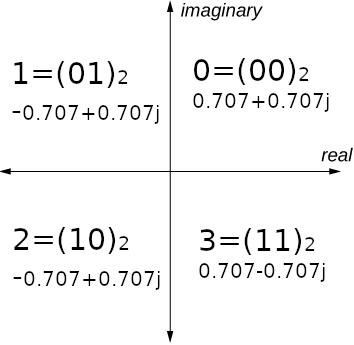
\includegraphics[width=0.75\linewidth]{mapping_qpsk.jpg}
            \caption{QPSK: Mapping Symbols to Constellation Points}
            \label{fig:mapping_qpsk}
        \end{figure}
        
        The last block is "Throttle", to understand this block we need understand how GR works: when we do data streaming we are implicitly using buffers to hold the data between blocks, this buffers are in finite size, so before the block do anything, it checks the amount of available space in input and output buffers, if there is none available space in that buffers the block don't do anything. This is called "Back-pressure" because we pressure back the data that is incoming, slowing things down. This is how GR controls the data flow, giving data to the block when it's necessary and holding it when block is busy working. We have source/sink blocks that produces/consumes data at a given fixed sample rate like Audio and USRP blocks, these blocks are called "clock" blocks, so typically an FG has only one source or one sink block, and not both because that leads to an problem called as "2 clock problem" where there is 2 blocks with different sample rates leading a asynchronous clock sources causing "underruns"/"overflows" depending on the production/consumption rates are differentiating. As our FG doesn't has any of this "clock" blocks then we need to add the "Throttle" block to act as a clock, without it the FG will run as fast as the CPU can process resulting in non-responsive program and other problems. This means that while we are in simulating mode we need this block to control the flow however when we start using the "USRP" blocks we can take out this block.
        
        To finalize the TX side we send the data to an "Virtual Sink" block, that redirects the data to the "Virtual Source" block with the same ID, the only purpose of this block is making the FG more clear, elegant and readable.
        
        Now we move to the RX part where we can use one of two decoders, an hard decoder or a soft decoder. They both receives the complex values of the signal, however the hard decoder maps into bits of the symbols already set to use, while a soft decoder maps into a probability of the bit being 0 or 1  (decision based on the LUT table in constellation object), hence, we can convert this probability into real bits (using "Binary Slicer" block or sometimes it's useful use soft bits for example when using "Forward error correction decoder" block. 
        
        We will move on with the hard decoder, so we use the "Constellation Decoder" to invert what we have done, this is, map the complex points to hard decision symbols (using the parameters of the the "Constellation Object" block), and then we use "Map" block again to map symbols into bits of real data. And then pick the 2 significant bits and pack in a byte exactly the inverse that we did before.
        
        
\subsection{Modulation - Tutorial\_2.grc}
    What we have done is not enough because in real world we cant use all the bandwidth, so we need no narrow it, however if the channels are too narrow the symbols will be too wide and the tail of the last symbol will interfere with the present one inducing ISI (Inter-Symbol Interference). A pulse shaping filter we can use to work around is the RRC (Root Raised Cosine) filter because it's a feasible solution and it's already implemented in GR.      
    
    %--------RRC filter
   If we don't put a shaping filter on the signal, the waves will have a lot of energy in adjacent channels. This filter uses taps to apply against our signal shaping it. This taps are calculated based in how many number of filters we want and how many samples we want per symbol. Theoretically has an infinite number of taps hence we can infinite attenuate the stop band, so really we can define the limit according with processing power we have. Remember that we have added ISI here that we will have to treat in RX side, as we will see.
   

    %Roll off
    
    Another thing to keep in mind is the roll-off factor, this is the measure of the excess bandwidth of the filter (bandwidth that is occupied beyond Nyquist bandwidth). This parameter is basically the inclination of the wave when rising and falling, when we set more roll-off, let's say 1, then will be easier for the receiver to decode however we will narrow less the bandwidth and that is not our objective, on the other hand, smaller roll-off will result in narrower bandwidth, however the inclination increases so attenuation in stop band is reduced.
    I provide an FG that I have made called \verb|roll_off.grc| inside of \verb|Extra| folder where you can analyse the plot of 5 different roll-off factors. In this tutorial we will use the 0.22 value to this parameter for being the middle ground in terms of trade-off, hence, the most used for communication systems.
    %-filter delay.
    %--Decreasing the number of samples (filter delay) reduces the stop band attenuation.
    
    %---SPS
    Another thing included in modulation is the interpolation which is increase the SPS (samples per symbol), so basically we can set a number of SPS that we want and more samples per symbol leads to less probability of errors, however, logically we are inducting more overhead to our transmission (we are transmitting more information). What this does is construct new points in the wave between the existing ones thereafter when we will reconstruct the signal we will be a lot more precise. To find this parameter we have 2 criteria:  First leaving this values small as possible taking into account that is mandatory to be 2 or higher. Second we can use this value to help us match the desired bit rate taking into account the sample rate of the hardware we are using (currently none but we will use USRP's). We will use 4 for this parameter.
    
    %--------RX SIDE - chega??
    Note that at this point we have ISI in our signal, so first we have to get rid it. When we combine 2 RRC filters together we get a RRC filter with Nyquist filter form. Knowing this property we can use another RRC filter resulting in a raised cosine pulse shaped filter with less ISI. If you observe the constellation plot "RX Treated Constellation" there is a little noisy as a result of the ISI after the 32 filters however much less noisier than "RX Constellation". 
    %--SPS 4-1
    
    Now that we have applied a RRC filter to our RX signal, in the same way that we have interpolated by 4 we need decimate to converting 4 SPS into just 1.

\subsection{Modulation - Tutorial\_3.grc}
    Now we are ready no get closer to reality, for that let's implement a "Channel Model" block where simulates different properties of a channel that we will need to take care:
    
\begin{itemize}
\item Noise - We can add Additive White Gaussian Noise (AWGN) in parameter "Noise Voltage" where we set a level as a voltage;
\item Frequency Offset - The "Frequency\_offset" parameter where 0 is no offset and 0.25 would be a digital modem (1/4 of the symbol rate);
\item Timing Offset - The "Epsilon" parameter allows emulating different sample clocks between the transmitter e the receiver and 1.0 is no offset added.
\item Multipath - We can emulate multipath delay by adding taps of a FIR (Finite Impulse Response) filter in the "Taps" parameter.
\end{itemize}
    
    %---EXTRA-- e POLYPHASE
    I have added in \verb|Extra| folder an example named \verb|data_timming_offset.grc| where inputs some data and simulates an offset clock, then you can see that the data has different arrival times, this is timing offset, and we need to take care of this in our main FG. Fortunately we already do it (and noise too) by using the "Polyphase Clock Sync" block. 
    
    
    %O que é multipath - tratar MULTIPATH
    Multipath is having different paths to our receptor like when we are using wireless where the signal reflects on environment objects, for example walls, and go to receptor a little after of the direct path signal, so the receptor receives the same signal various times with slight timing differences. 
    If you bypass "CMA Equalizer" block, enable the first taps variable (which is with almost no taps) and set "Output SPS" to 1 in the "Polyphase Clock Sync" you can play with the tweaks "Time Offset" and "Noise Amp" and you can see in the plot labeled as "Rx Treated constellation" a nice and clear constellation (although a little rotated). Now only enable the second taps variable which I added to simulate a multipath property and run you can now see the effect of these taps because the constellation points are no longer clean and really converged: Figure:  \ref{fig:multipath_effect}
    
    \begin{figure}
        \centering
        \includegraphics[width=\linewidth]{multipath_effect.png}
        \caption{Effects Multipath on Constellation Plot}
        \label{fig:multipath_effect}
    \end{figure}

    This obviously affects our transmission, so to take out this problem we will need an equalizer, called "CMA Equalizer". Here we define the number of taps where more taps means better final results however more overhead to the algorithm, thus, we want keep this number small but enough for correcting our channel (based on educated guess, and some experiments I have set 15). The "Gain" I have set 0.01 and the "Samples per Symbol" of the input signal I want set to "2", hence, the "Output SPS" of "Polyphase Clock Sync" block is also set to "2". If you take a look now for the constellation plot you will see a constellation a lot more converged and clean: Figure: \ref{fig:multipath_corrected}

    \begin{figure}
        \centering
        \includegraphics[width=\linewidth]{multipath_corrected.png}
        \caption{Multipath corrected on Constellation Plot}
        \label{fig:multipath_corrected}
    \end{figure}
    
    Note that the constellation is rotating a little, the "CMA Equalizer" all it cares about is converging in a unit circle without any knowledge of the constellation, so when it locks, locks in a given phase, thus we need to take care of the phase offset (or frequency offset). Besides that if you tweak the "Freq Offset" you can see that the constellation become a circle, that's because we are not treating the frequency offset, it will be what we will do in the next tutorial.
    
\subsection{Modulation - Tutorial\_4.grc}
    %TRATAR Frequency offset - COSTAS LOOP -------__MELHORAR??????????
    There exists two types of frequency correction, the fine frequency correction and the coarse frequency correction. We will start by treating the first one, this is, we can track the offset by using an second order loop when our signal is close of the ideal frequency or our constellation won't converge and will keep spinning. For this we will use a "Costas Loop" block where we have to set the "Loop bandwidth" and the "Order" parameters, the first one is relative to the second order loop (I will use 6.28/100.0 which is recommended, this value adapts to the signal in runtime), the second is about the order of the constellation type (2 to BPSK, 4 to QPSK and 8 to 8PSK, thus, 4 for our example). Now if you disable the "FFL Band-Edge" block and run the FG you will note that the constellation is no more rotating and if you tweak the Frequency Offset note that it's not getting a circle anymore, instead that, the constellation keeps without rotation, clear and converged. 
    
    %COARSE FREQUENCY OFFSET CORRECTION
    But, as I have said we have done fine frequency correction so if you continuously keep increasing the "Frequency Offset" tweak you will see that at certain point (close to 0.034) the constellations starts to be a lot noisier. Now we need to take care of "Coarse frequency recover" using "FFl Band-Edge" block. This block uses a frequency lock loop that derives of an band-edge filter that covers both upper and lower bandwidths of the signal to keep it in a range determined by the roll-off factor. This factor together with the SPS positions the frequency of band-edges.
    Concluding, first we set the SPS by 4, the roll-off factor at 0.22 as previously discussed. We also need to set a number of filter taps that we will generate to apply to our signal (I have set 60) and then the loop bandwidth (I have set 6.28/400.0). If now you tweak the "Frequency Offset" beyond what "Costas loop" alone can handle you see a perfect and clean constellation. 

\subsection{Packet communications - Tutorial\_5.grc}
    %---Header e CAC
    Now we have successfully modulated and transmitted our signal, but if you take a look in the output file, it will only be junk. This is happening because it's not writing the bits in the supposed byte. Explaining better, if I send the byte "01010101" and for some motive receives 4 bits in 0's and then the right byte, this results in "0000\textbf{0101}" and "\textbf{0101}XXXX", then all the bits forward are not aligned. This is the problem that is happening here because the "Polyphase Clock Sync" block needs some time to adapt and in this time write some junk bits, so we need a manner to always receive the bytes aligned. The solution for this is packetize our data and send the packet, consequently, we will lose all that first packet but we will always get our bits aligned.
    
    %CAC
    The first thing we need to know is how the "Correlate Access Code - Tag Stream" block works. It expect unpacked data, this means that the input only has 1 significant bit per byte. Then exams the input finding an sequence called "Access Code" of 64 bits taking into account that can be X bits different where X is the "Threshold" parameter. After find this sequence the next 16 bits is the length of the payload (that will be outputted) repeated twice (32 bits in total). Resulting in a header with 64 bits of access code, 16 bits of payload length and another 16 bits of payload length, being that the length of the payload is in bytes. Now that we have the composition of the header of the packet we need to create it.
    
    %Inicio
    Assuming that we want transmit packets with 112 bytes of payload size, hence 896 bits, then we need to create the header with that information. 
    %-Create header
    To create the header we will use the "Vector Source" block with the "Repeat" parameter set to "Yes", and the vector will be 64 bits of the access code (I will use the default that can be accessed here "digital.packet\_utils.default\_access\_code"), followed by "00000000 01110000" = 112 and then "00000000 01110000" = 112. With header ready we need to split the input in 1 bit/byte using "Repack Bits" block mentioned before, then concatenate the 96 bits of the header with 896 bits of the payload using "Stream Mux" block, and finally repack again to 2 bits/byte resulting in the packet ready to modulate and transmit. Of course that this can be optimized by instead repacking into 1 bits, uses directly 2 bits and creating the header with that in mind, but I am splitting in 1 bit because we will use FEC (Forward Error Correction) encoding ahead.
    
    %RX
    At the RX side we just need to repack to the 2 bits/byte into 1 bit/byte to use the "Correlate Access Code - Tag Stream" block and extract the payload of the packet and finally repack to 8 bits/byte. Now if you take a look at the output file you see that the bits are aligned correctly in the byte needed.
    
\subsection{Out-Of-Tree Modules - Tutorial\_6.grc}
    We are getting the bits aligned, but we lose the first packet so we can solve this by transmitting an vector of bits right before we transmit our real data. There is just a big problem: The GR doesn't has that implemented but has a thing called OOT (Out-Of-Tree Modules) where allow us extend GR with our own functions and blocks created in Python or in C++. Now I will teach how to create a block in GR: The first thing to do is go to an folder where you want keep the OOT blocks and run the following commands: 

\begin{lstlisting}[language=bash, breaklines]
$gr_modtool newmod insert_vec_cpp
$cd gr-insert_vec_cpp
$gr_modtool add new_vec
\end{lstlisting}

    Now we need to chose the type of block we want to write, where:
    \begin{itemize}
        \item Source - With this blocks you can produce output items.
        \item Sink - With this blocks you can consume input items.
        \item General -This block is a general version, where you can define the rate of consumption/production. 
        \item Interpolator/Decimator - Use this type when you want a fixed multiple rate of consumption/production.
        \item Hier - This is called "Hierarchical blocks" where you can aggregate multiple existing blocks in one block. You can also do this in a graphical way on GR by setting the parameter "Generate Options" as a "Hier Block" located in Options of the FG.
        \item No Block - You can also create FG without any graphical blocks, only code.
    \end{itemize}
    
    For our purpose I selected \verb|general|, and then we need to select the language (it can be in Python or C++), I have selected \verb|cpp| as the language, then you need to input the arguments that your block will take, as I want only an vector of bytes I put \verb|const std::vector<unsigned char> &vec|, and  finally you select if you want QA (Quality Assurance) code, this is a template where you can do unit testing on your code (I selected no).
    
    Here it's created 3 important things:
\begin{verbatim}
File 'lib/new_vec_impl.h'
File 'lib/new_vec_impl.cc'
File 'grc/insert_vec_cpp_new_vec.xml'
\end{verbatim}

    The first one is the header file of our source code file witch is the second file and where we will write our code. The last one is an XML file where we link our code to the GR.
    
    %---CODE
    Let's carefully analyse the source file, in the constructor we have:
\begin{lstlisting}[language=c++, breaklines]
gr::io_signature::make(<+MIN_IN+>, <+MAX_IN+>, sizeof(<+ITYPE+>)),
gr::io_signature::make(<+MIN_OUT+>, <+MAX_OUT+>, sizeof(<+OTYPE+>)))
\end{lstlisting}

    The GR adds \verb|<+| and \verb|+>| in places that you need to replace for values that you need. The first line is where you select how many input connections you need, namely the minimum number, the maximum number, and the size of the type of data that will be on that connections. In our case we want to get in only one connection (so min=1 and max=1) and treat like a byte, this means that we need to set an \verb|unsigned char|.
    The second line is where you select how many output connections you need, namely the minimum number, the maximum number, and the size of the type of data that will be in each connection, so it's exactly the same as before.
    
    Besides that we will need to add some other things here, for example we need to use our vector in another function (general\_work) so we need to set it here, another variable is an flag to know if all the vector was sent and finally an index to track how many bits of the vector we already sent.
    Resulting in changes in file source and header file, in file source just add this:
\begin{lstlisting}[language=c++, breaklines]   
gr::io_signature::make(1, 1, sizeof(unsigned char)),
gr::io_signature::make(1, 1, sizeof(unsigned char))),
d_data(vec),
flag(0),
track_oo(0)
\end{lstlisting}  

    In header file declare the variables:
\begin{lstlisting}[language=c++, breaklines] 
    std::vector<unsigned char> d_data;
    int flag;
    int track_oo;
\end{lstlisting} 
    And make getters and setters:
    
 \begin{lstlisting}[language=c++, breaklines]   
void set_data(const std::vector<unsigned char> &vec){
    d_data=vec;}
int get_flag(){
    return flag;}
void set_flag(){
    flag=1;}
void set_track(int a){
    track_oo=a;}
int get_track(){
    return track_oo;}
\end{lstlisting}    

    The next function to treat in file source is this one:
\begin{lstlisting}[language=c++, breaklines]   
teste_impl::forecast (int noutput_items, gr_vector_int &ninput_items_required){}
\end{lstlisting}
    
    Here is where you define the production/consumption rate you want. We will want 1:1 so you need to add this in that function:
    
\begin{lstlisting}[language=c++, breaklines]    
unsigned ninputs = ninput_items_required.size();
for(unsigned i = 0; i < ninputs; i++)
    ninput_items_required[i] = noutput_items;
\end{lstlisting}
    
    Moving on for the core work \verb|general_work()| that will be performed by the block, the template show us this:

\begin{lstlisting}[language=c++, breaklines]    
    const <+ITYPE+> *in = (const <+ITYPE+> *) input_items[0];
    <+OTYPE+> *out = (<+OTYPE+> *) output_items[0];
    consume_each (noutput_items);
    return noutput_items;

\end{lstlisting}

    Again, we need to replace content of the \verb|<+| \verb|+>| for our type of data: \verb|unsigned char|. The consume\_each() function is where we set the number of items that we will consumed and at front of the return is the number of items that we produced.
    
    Going for the code itself:
    If all the vector was already inserted, then we just pass through the items doing nothing to them, using the \verb|memcpy()|.
    If there is the first time or vector to send then we need to send it, taking into account that we can only send the maximum size available on the output buffer. In case there is not enough space we sent what we can and update the variable to keep track of the last byte sent and next time we know where we will start sending the vector. Here we don't consume anything, we are just producing items. In case there is enough space then we sent the rest of the vector and set the flag to know that we already sent all the vector and starts passing directly the next items.
    So in \verb|general_work()| we will add this:

\begin{lstlisting}[language=c++, breaklines]
int ii=0;
int oo=0;
if(get_flag()==1){ //Vector already inserted
    ii=noutput_items;
    oo=noutput_items;
    memcpy(&out[0], &in[0], sizeof(unsigned char)*noutput_items);
}
else{ //First time or vector not fully sent, so I need to insert the vector
    int max_copy = std::min (noutput_items, (((int) d_data.size()) - get_track()) ); //Check for space in buffers to use the remaining vector (len(vec) - used)
    oo=max_copy; //That's what I will output (produce, it can be all vector or all buffer)
    ii=0; //I don't want consume anything
    memcpy(&out[0],&d_data[get_track()],sizeof(unsigned char)*max_copy); //Output starting from where I stopped the last time (Starting with 0)
    if(max_copy == (((int) d_data.size()) - get_track()) ){ //If I will use last piece of the vector (len(vec)-used) then I can set the flag to get out. (Start passing directly)
        set_flag();
    }
    set_track(get_track()+oo); //Increment the track to know where to start copying the vector the next time (Where I was plus what I will produce now) 
    }
consume_each (ii);
return oo;
\end{lstlisting}

%-XML
    In remaining file we have a XML where we need to set some things so we can link our written code to GR. The first tricky thing is remove the \verb|&| on the parameter in \verb|<make>| tag. 
    In \verb|<param>| is where we define the parameter that will be parsed in our GR, so we will replace this piece of the template for this:
\begin{lstlisting}[language=xml, breaklines]
<param>
    <name>Vector</name>
    <key>vec</key>
    <type>int_vector</type>
</param>
\end{lstlisting}
    Then in \verb|<sink>| and in \verb|<souce>| has a parameter called \verb|<type>| where we set what type of data will be inputted and outputted, in this case will be \verb|byte|.

    Now that we have all code written we need compile it and link to our GRC with these commands:
    
\begin{lstlisting}[language=bash, breaklines]
$mkdir build && cd build
$cmake ../ && make
$sudo make install
$sudo ldconfig
\end{lstlisting}
    
    Finally we just need to click in "Reload Block" in the GR's toolbar and use the block like any other. To create a vector we can use a "Variable" block and use the Python input \verb|[int(random.random()*X) for i in range(Y)]| where X is the alphabet of the vector (I want between 0 and 3), and Y is the length of the vector (Value that needs to be experimentally found until starts transmitting well our data).
    
    If you prefer, instead doing manually all this code, I let you the all OOT ready to use in \verb|Extra/OOT/Insert Vector|, you can just unzip it and run \verb|/script.sh| inside \verb|build| folder. To uninstall the OOT you need to do it manually by running \verb|sudo make uninstall| in the same folder.
    
\subsection{Forward Error Correction - CC - Tutorial\_7\_CC.grc}
%-----Intro
    In a wireless transmission, obviously, we may have transmission errors, so we need to take care of some of these errors by using some error correction. The GR offers a module called FEC (Forward Error Correction) where exists three encoding blocks: "FEC Encoder", "FEC Extended Encoder", "FEC Tagged Encoder" and "FEC Extended Tagged Encoder". They all expect bits (generally soft decisions, this is, values between -1 and 1) and produce bits (real bits, this is, 0 or 1), this means we need do work with unpacked bytes however there is only a few differences between them: the first one only inputs the data and outputs a bigger stream the data (added of redundancy), the second one it's a wrap (a heir block) of the first where is added puncture (common in this type of encoding), and properly convert the input/output data. The third one, instead using the Frame Bits defined in the encoder object block for knowing how many bits it's inputed to FEC, uses a stream already tagged and automatically increases the length of that tag, finally, the last one is similar to the third however takes care of puncture and some data conversion. All of them uses as a parameter an encoder object which determinate the type of encoding we will use, this object can the one of these encoding types:
    \begin{itemize}
        \item Dummy Encoding - The dummy encoding simply redirects the input to output with no error correction. This simply allow us to use and test the the encoder block.
        \item Repetition Encoding - This encoding only repeats the same bit how many times we define, thus, has a low performance taking into account that we multiply the amount of bits needed to transmit.
        \item Convolutional Code - This code generates parity symbols by sliding and polynomial function to our data stream. Here we can use 2 blocks, or the "CC Encoder Definition" object which is an generic implementation where it's prepared to use different polynomials, rate and constraint lenght (currently the GR has only implemented the Voyager code from NASA), or use the "CCSDC Encoder Definition" object which is an highly optimized implementation of the Voyager code.
        \item LDPC (Low-Density-Parity-Check) - Here we have two types that we can use, or we use an already created Matrix (using "LDPC Encoder Definition (via Parity Check)") or we use an Generator Matrix (using "LDPC Encoder Definition (via Generator)").
    \end{itemize}
    %-----_EXTRA BER CURVE-----------
    I have added an example (not created by me, found here: \url{https://github.com/gnuradio/gnuradio/tree/master/gr-fec/examples}) in \verb|Extra| folder called \verb|ber_curve_gen| where you can analyse the BER (bit error rate) curve in different FEC types. I advise you to run directly from console using python to avoid some problems.
    %----Implementation
    I will implement the convolutional code using the "CC Encoder Definition" object block to extend the life of this tutorial. As I have told, the "FEC Extended Encoder" expects unpacked bytes so before we send data to that block we need to repack the bits from 8 to 1, and then we can use the block. Now we need to fill the parameters, first we set a puncture pattern of '11' (where there is no puncture), then the "Threading Type" parameter we set to "None" for now (I will be back here). Regrading to the "Encoder Object" we will use the "CC Encoder Definition". This block has a lot of important parameters: The Frame Bits" tells how many bits we want to input of each work (I will set for our example 440 bits).The "Constraint Lenght (k)", the "Rate Inverse (1/R)", and the "Polynomials" I have set "7","2" and "[109,79]" which is the Voyager Code and the only available code at this moment.
    At "Streaming Behaviour" we have four options:
    \begin{itemize}
        \item Streaming: Expects uninterrupted flow of bits to the encoder, where the output is continually encoded.
        \item Terminated: Used for packet-based, however this mode adds "rate*(K-1)" bits to the output to help flush the decoder.
        \item Tailbiting: Used for packet-based, however instead adding bits, uses the final bits of the packet when we are decoding.
        \item Truncated: Here the registers are reset between frames.
    \end{itemize}
    
    Another important thing to keep in mind is that I want send the encoded packet independent of the last one, so if I lose one packet I don't start a chain of corrupted packets. 
    
    Taking in this into account, we can possible we 2 of this modes,the "Terminated" or the "Tailbiting", however I want the packets fully independents of each other so that if I lose one packet I don't start a chain of encoded packets, thus, we will use the first mode.
    
    With all this our output of the encoder will be the input multiplied by rate plus the added bits to flush decoder resulting in: (Input * Rate) + (Rate*(K-1) = 440 bits * 2 + (2*(7-1)) = 892 bits.
    
    Now that we have the payload encoded we just need to create the proper header exactly as before, but we have a problem here: in the header we need to define the payload in bytes, however, we can not convert 892 bits in bytes (892/8=111.5 bytes). To solve this we need to add 4 bits resulting in 896 bits, or 112 bytes converted. We can add this using a "Vector Source" Block concatenating the vector with a "Stream Mux" block. All this step can be visualized in Fig: \ref{fig:multipath_corrected}
    
    We can now transmit our packet with the payload already encoded. In reception all we have to do is do the inverse that we have done by using the "FEC Extended Decoder" along with "CC Encoder Definition" object and then only keeps the firs 892 bits of 896 bits with the  "Keep M in N" block. Note that the decoder blocks now uses soft decision bits (floats between -1 and 1), but as we have an hard decoder we get hard decision bits (0's and 1's), so we just need to Map and  then use the "Char to Float" block.
    
    If you run the FG and look at the CPU processing you can see that only one thread is running slowing down our FG, so we can use multithreading by creating multiple encoder variables with same settings defined in "Parallelism" parameter of the encoder object. This value can be 1 or 2, where 1 creates a list of variables and 2 create a list of lists of variables. The length of that list is defined in "Dimension 1" parameter also there. The "FEC Encoder" block must know how to handle with these variables, for this we can set one of the two options: "Capillary" or "Ordinary" in parameter "Threading Type". The difference between them in N streams and pass each N stream to one encoder variable to process the frames in parallel and then the output of each variable is interleaved back together making a single stream. The second one is like the another however it creates a tree where each branch launches 2 more branches, thus N must be a factor of 2. This perform better than the other. With this in mind I have set to 1 in "Parallelism" and create 4 variables to the encoder and 8 variables to the decoder because the decoder it's less efficient than the encoder.
    

\subsection{Forward Error Correction - LDPC - Tutorial\_7\_CC.grc}
    I have added an example (not created by me, found here: \url{https://github.com/gnuradio/gnuradio/tree/master/gr-fec/examples}) in \verb|Extra| folder called \verb|ber_curve_gen_ldpc| where you can analyse the BER (bit error rate) curve in different LDPC types (Parity check and Gen. matrix). I advise you to run directly from console using python to avoid some problems.

    Like I have told there is two types of LDPC implementations, I choose to use the "LDPC Encoder Definition (via Parity Check)" and pick a matrix already given by GR. Where for each 442 bits results in 1100 bits. Here I need to give to "FEC Extended Encoder" block 442 bits of data to work, however I want send full bytes but 442 bits it's 55.25 bytes. An work around of this is simply pick 440 bits of data (55 bytes) and add 2 bits just for complete the necessary amount of bits to LDPC work. Hence in the RX side we need to add a "Keep M in N" block where we only keep the first 440 bits of data. The rest of the FG it's analogue to the CC's FG with just some changes about the values of header and the stream mux blocks.
    
\section{GUIDED TUTORIAL - FULLY WIRELESS}
\subsection{USRP - Tutorial\_8.grc}
    Now it's time to get fully wireless, for this we will remove all the part of the channel model and add an "USRP Sink" block and an "USRP Source" block. Like I have told in tutorial\_1, note that now we can remove throttling because we will have an "clock" block that consume/produce data at an fixed sample rate. I also told that we can't have 2 "clock" blocks or we would have the "2 clock" problem, this is totally true but as this blocks are physical both parts of TX an RX will be totally independent not back-pressuring data thus not changing sample rates.
    
    To got the FG working you just need to change the parameter "Device Address" for your USRP serial which can be found running the command \verb|uhd_usrp_probe|. 
    
    When we change from simulation to real world we introduced an problem called "Saturation Limits", this is, the "USRP Sink" needs to send floating values between -1 and 1 anything below or above is bad causing the signal to be saturated and nonlinear which we don't want of course. We can visualize this by adding an Time Sink (which I already did) and now if you bypass the "Multiply Constant" block you will see in "TX USRP" time sink a lot of values out of the limits, this is why we need to add that block defining the multiplier value by trial and error until we get nice values inside of the limits. However this block doesn't solve for the RX side, for this enable again the previous block and run the FG and play around with the TX/RX gain, once you find good values you can define these values in the correspondent variable blocks. If you don't change the positions of the USRP's and the antennas this should work well.
    
    Now that we are providing good values to the USRP's we need to tweak the sample rate in a form that can be the maximum possible (for higher speed) however without drop data. We may have two problems here, it can be printed U' and/or O's in our console. The U's means "Underun", which means that in TX side we are not giving samples enough quick to our USRP to send them, this can be caused for lack of processing power (note that the encoder block requires a lot of power) so what we need to do is: or we change the CPU or we slow down the sample rate of the USRP's. When we have 0's this means "Overrun", this is, in RX side we are not able to consume samples quick enough, probably because of the back-pressure caused by the decoder block. So we need to found the maximum value for the sample rate taking into account 2 things: If it prints U's or 0's, there can be only in beginning because of rampage up, this is here another reason for adding and vector previously sending our real data, so we lose data of the vector and not data of our transition data. Another thing is that we must choose an sample rate where \verb|clock rate/sample rate| must be an integer, and for better performance should be divisible by 4.
    Taking this into account I improved the MCR (Master Clock Rate) of the USRP for 60e6 and I have created an vector with sample rates that are best for performance, thus, we just need to choose the index on the vector to change the sample rate.

\subsection{USRP - Tutorial\_9\_Differential\_Encoder.grc}
    %Problema
    If you take a look to the "RX Data" plot you can see that we have a problem writing the data, sometimes it does and other times doesn't. That's because we have phase ambiguity for some amount due to the presence of phase distortion in communication channel, we can have 2 possible orientations for BPSK (180 degrees), 4 possible orientations for QPSK (with 90 degrees), M orientations for MPSK (with 360/M degrees), in our case we have of 90 degrees in our constellation. 
    
    %-2solucoes. Explicar vantagens e desvantagens differential
    There is two solutions for this: The first one is using an already known signal to train the receiver by correlating it with the outputed signal and get the real phase, this will be done in the next section. Another solution for this is instead transmitting the direct mapping in symbols into the constellation, we will transmit the difference between symbols of the constellation using the differential encoding where a symbol depends not only of the transmitted symbol but also the previous one (\verb|y[0] = (x[0] - x[-1]) % M| where M is Modulus of code's alphabet), removing the ambiguity. As everything else we have pros and cons in the use of one or another, the advantage of differential encoder is that there is no need to train the receiver, hence it's faster because we are not introducing overhead, however, as a disadvantage, if occurs one error in the transmission can cause two symbols wrongly recovered (because the dependency of the last one).
    
    In our FG we will remove the "Map" block, since it does nothing now (because we cant use other map than \textit{[0,1,2,3]} or we will take out the difference of symbols), and we will add an "Differential Encoder" Block right before "Chunks to Symbols" block resulting in conversion the input symbol in a one dependent of the last and thereafter it's mapping in the constellation point. 
    In RX is just do the inverse thing, right after we decode the symbols then we apply the "Differential Decoder" to retrieve the original symbols.
    
\subsection{USRP - Tutorial\_9\_Correlation\_Estimator.grc}
    %
    As I said we always have pros and cons, about the "Correlation Estimator" the main advantage is that we can use Gray Coding, this is, we have at maximum 1 bit of difference between adjacent constellation points. In Figure \ref{fig:gray_coding.png} it's easy understandable the difference between Natural codding and Gray coding maps (note that we can use gray coding also in 8PSK). With Gary Coding if the transmitted signal is mapped in other adjacent constellation point only will transmit 1 bit of error and not the all symbol, hence more easy to the FEC correct the error. In other hand, we introduce more overhead to our FG because we need more computing power to correlate the signal with our sync word.

    \begin{figure}
        \centering
        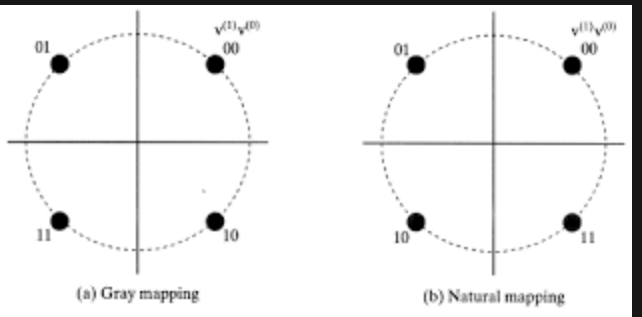
\includegraphics[width=\linewidth]{gray_coding.png}
        \caption{Natural Coding Vs Gray Coding}
        \label{fig:gray_coding.png}
    \end{figure}
    
        %explicaro o bloco e as tags
    
    The "Sync Word" is a set of known bits both by Tx and Rx, so if the Tx sent them, the Rx is capable of identify this sequence and do something with that. The identification method used is a property called correlation where we correlate the inputed signal against this word and then creates a peak of energy that can be used for estimate several things. To this work we need a sequence with low auto-correlation in all the points except in the central one, being in this manner strong against noise (it can changes some bits). For this sync word exits already known sequences for example the "Barker Codes" (with 13 bits of maximum length), however we need a bigger sequence for higher peaks so we will use the default access code, where the result of auto-correlation it's showed in the Figure \ref{fig:correlate_ac.png}, besides that, as it's the same known word for the header of the packet we don't increase the amount of data transmitted.
    
     \begin{figure}
        \centering
        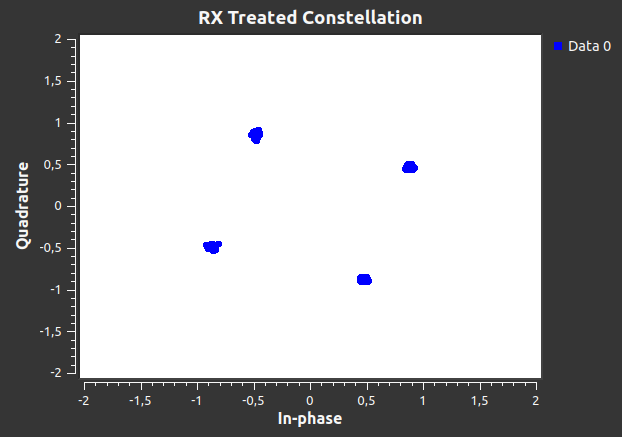
\includegraphics[width=\linewidth]{correlate_ac.png}
        \caption{Auto Correlation}
        \label{correlate_ac.png}
    \end{figure}
     

    With the "Correlation Estimator" block we can do exactly what I said, so we input the signal containing the sync word and correlates with the sync work resulting in estimations. The bock outputs the exactly same input however has tags attached, like:
    \begin{itemize}
    \item phase\_est - Estimated of the phase offset, used by the "Costas Loop" to reset it's internal phase value and speeds up the synchronization, removing here the phase ambiguity.
    \item time\_est - Estimated of the timing offset, used by the "Polyphase Clock Sync" to synchronization.
    \item corr\_est - The values resulted of the correlation.
    \item amp\_est - Estimated amplitude, it can be multiplied my this value before get in the Polyphase Clock Sync.
    \item corr\_start - The start sample of the correlation and the correspondent value.
    \end{itemize}
    
    Going to the parameters, first we need to set the "Symbols" parameter which is the "Sync word" already modulated, so we use a block called "Modulate Vector" where we input one vector and modulates it applying the filter taps parameter. The modulator we will use will be the generic with the right parameters, namely, the constellation object, "false" to differential encoder, then our SPS, then "true" for using the map of the constellation object, then the excess bandwidth we used to modulate the signal, then "false" for verbose and finally another "false" for logs, resulting in:  \texttt{(digital.generic\_mod(pld\_const, False, sps, True, eb, False, False))}. Note that this generic modulator take packed bytes, so we need to create a vector of packed bytes of the 64 bits access code, and applies already the RRC so we don't nedd to do it in the "Filter taps" parameter 
    
    There is tricky thing here because there exists a delay in the correlation detection algorithm (affected by the size of the sequence) then we need to adjust the place where they are actually placed on the stream, we can do this using the "Tag markinig delay" parameter which is influenced by the SPS and sequence length. This value is found empirically by tweaking the values and analysing the second output of this block.
    
    Finally the "Threshold" parameter is where we define how much precise we want relative to a 100\% correlation, so set values between [0-1], I have set 0.999 because it worked well, however if it's not working for you try to decrease this value. Note that you can see the correlation working in "Correlation" and "Correlation  \^\ 2" plots.
 
\subsection{USRP - Tutorial\_10.grc}
    It's everything working perfectly when we are using random bits however if we input a file with some zeros in a row, the FG losses symbol synchronization, for example you can easily testing by inputting the \verb|videofhd.mpeg| file provided. As you can see in output the zeros are not transmitted well, so we need to somehow instead transmit all this zeros in a row, transmit it with some bits at 1 without adding significant overload to FG (by increasing the amount of transmitted bits). A solution for this is adding a scramble block and the after all the transmission undo what we did.
    
    
    %------------FALTA---------------------
    %---Explicar funcionamento LFSR - Scrambling
    The scramble it's often used to improve security in a transmission, however, at this view has nothing related with that but aims to eliminate long sequence of same bits (called whitening sequences), consequently reducing problems with synchronization at the receiver. A Multiplicative Scrambler works using an LFSR (linear-feedback shift register) which is a shift register whose input bit is a linear function of its previous state. We have mainly two parameters, the number of registers, N, which primarily contains a value called "seed" and is updated for each state where the output bits are determined taking into account the current and the previous state of these registers (because of their operation is deterministic). Just some of the registers influences the output, this are called taps, to know which ones we need to determinate a polynomial of type \(x^a + x^b + ... + x^z + 1\) where the register number \verb|a,b,...,z| are the taps. The 1 corresponds to the input of the first bit (note that is \(x^0\)). For each iteration receives an input bit, is XOR'd with the content of the taps, and then all registers are shifted to the next register, being the last one discarded, we can visualize this in Figure-TIRAR ESTA(da net) E POR UMA MINHA: \ref{fig:scramble}
    
    \begin{figure}
        \centering
        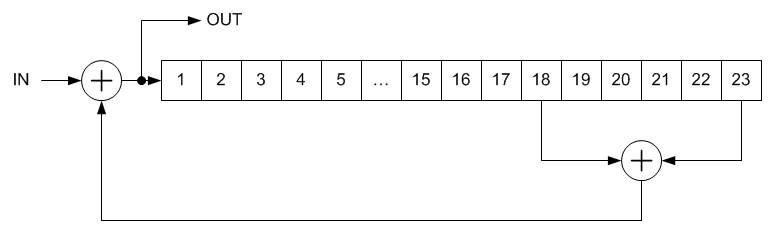
\includegraphics[width=\linewidth]{scrambler.png}
        \caption{Scramble}
        \label{fig:scramble}
    \end{figure}
    
    
    %-Descrambling
    After we have the stream scrambled and we need to restore the original stream, for that we just do the reverse thing that we have done, so, for each iteration of input bit, the output bit is the difference between that bit and all tap bit's XOR'd between them. For more understanding please see Figure-TIRAR ESTA(da net) E POR UMA MINHA: \ref{fig:descramble}
    
    \begin{figure}
        \centering
        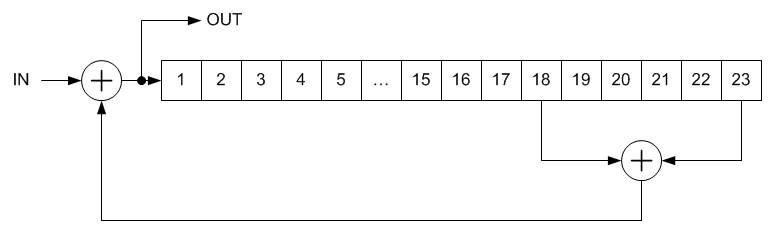
\includegraphics[width=\linewidth]{scrambler.png}
        \caption{Scramble}
        \label{fig:descramble}
    \end{figure}
    

    %--Examplo
    For better explanation, in practice, first we set a number of registers, let's say 7, and then we pick an polynom (there is a lot known), let's say the \((0X19)_{16} = (00011001)_2\ = x^4 + x^3 + 1\), so only the content of 4º and the 5º register influences the output, let's say X and Y respectively. For a given input bit B, the result that will add to the first register is: B XOR X XOR Y, and finally all bits are shifted to the next register. Always like this in successively. 
    %_--------------IMAGEM SCRAMLING E DESCRAMBLING
    
    
    %----Problema Scrambler Nativo
    We already have a native scrambler in GR that we can use we just drag and drop, however, the output bit of a LFSR is dependent of the last bits inputted like I said before, so if we lose some bits, we lose every single bit ahead. What we need to do to work around this is create a new scrambler that takes a piece of bits (a packet) and scrambles only that packet, and then reset the seed and scrambles another packet and so on, using always the same seed to initiate the registers. The descrambler is the same idea.
    
    Another problem that we face is that at first what we have in registers is the seed, so the first byte to output after the descrambler is only junk, and we don't output the last byte because it stays in the registers. To solve the first problem we just need to drop the first byte after we scramble, and then is the real data is transmitted. To solve the last problem we just need to flush the scrambler by inputting one more byte with 0's, so the last byte of the packet is transmitted as well.  
    
    %CODE
    Going to the code itself the idea like I said is create frames so for that we need to can reset the registers in the LFSR, if you go to installation folder of GR (if you followed my instructions should be here: \verb|/usr/local/include/gnuradio/digital|) and analyse the file \verb|lfsr.h|, you see an function called \verb|reset()| where reset the registers to the given seed. We will use it for resetting the seed before we scramble/descramble every packet.
    
    %--Explicar umbocado do codigo
    First we need to create an OOT like discussed before, i used \verb|scrambler_packets_same_seed| to the module and \verb|scramble_packetize/descramble_packetize| to the scrambler/descrambler blocks. Then in the code of the scrambler we have 3 branch that we can go, if it's the first bit of the frame, like I said before the first 8 bits are junk, so we scramble 8 bits but we don't send them, here we just consume samples we don't produce. If we go to the last bit of the frame, so we need to produce 8 more bits to flush the scrambler, here we just produce, don't consume, finally if we are in the middle of the frame basically we just check the output buffer space and we scramble everything possible (the size of the buffer or the size of the frame), consuming and producing.
    So we set flags for this 2 first branches and the code itself in work function it's this:
    
\begin{lstlisting}[language=c++, breaklines]
const unsigned char *in = (const unsigned char *) input_items[0];
unsigned char *out = (unsigned char *) output_items[0];
int ii=0; //Track how many input bits we consume
int oo=0; //Track how many output bit we produce
if(flag_last==1){ //It's the last bits of the frame: -> We need to flush it
    max_n_produce=(std::min(noutput_items,track_n_bits_added)); //Check buffer to the amount of bits that we can scramble
    for(int i=0; i<max_n_produce; i++){
      out[i]=d_lfsr.next_bit_scramble(0);
      oo++;
    }
    if(max_n_produce==track_n_bits_added){ //If we sent all bits: ->Reset variables ->Go to the first bits branch
      flag_last=0; 
      flag_first=1;
      track_n_bits_added=8;
    }else{ //If we didn't sent all bits, then go again to send what is possible. 
      track_n_bits_added=track_n_bits_added-max_n_produce;
    }
}
else if(flag_first==1){//First bits of the frame: ->Trash so we DROP
  d_lfsr.reset(); //Reset the registers using the seed
  for(int i=0;i<8;i++){  //DROP 8 bits
    d_lfsr.next_bit_scramble(in[i]);
    ii++;
    remaining_bits--;
  }
  flag_first=0;
}
else{ //Normal behaviour - Inside the frame
  max_n_produce=(std::min(noutput_items,remaining_bits)); //Check buffer to the amount of bits that we can scramble
  for(int i=0; i<max_n_produce; i++){
      out[i]=d_lfsr.next_bit_scramble(in[i]);
      ii++;
      oo++;
    }
    if(max_n_produce==remaining_bits){ //If we sent all bits:  ->Go to last branch to flush ->Reset variables
      flag_last=1;
      remaining_bits=n_frame;
    }else{ //If we didn't sent all bits, then go again to send what is possible. 
    remaining_bits=remaining_bits-max_n_produce;
  }
}
consume_each (ii);
return oo;
\end{lstlisting}
    
    In the descrambler we just use the function \verb|next_bit_descramble| in \verb|lfsr| to descramble the bits taking into account only the frame bits. Like this:
    

\begin{lstlisting}[language=c++, breaklines]
const unsigned char *in = (const unsigned char *) input_items[0];
unsigned char *out = (unsigned char *) output_items[0];
int ii=0; //Track how many input bits we consume
int oo=0; //Track how many output bits we produce
max_n_produce=(std::min(noutput_items,remaining_bits)); //Check buffer to the amount of bits that we can descramble
for(int i=0; i<max_n_produce; i++){
  out[i]=d_lfsr.next_bit_descramble(in[i]);
  ii++;
  oo++;
}
if(max_n_produce==remaining_bits){ //All bits of the frame was sent: ->Reset registers with seed ->Reset variables
  d_lfsr.reset();
  remaining_bits=n_frame;
}else{ //If we didn't sent all bits, then go again to send what is possible. 
  remaining_bits=remaining_bits-max_n_produce;
}    
consume_each (ii);
return oo;
\end{lstlisting}   

If you prefer, instead doing manually all this code, I let you the all OOT ready to use in \verb|Extra/OOT/Scramble|, you can just unzip it and run \verb|/script.sh| inside \verb|build| folder. To uninstall the OOT you need to do it manually by running \verb|sudo make uninstall| in the same folder.

\subsection{Figures and Tables}

\begin{table}[h]
\caption{An Example of a Table}
\label{table_example}
\begin{center}
\begin{tabular}{|c||c|}
\hline
One & Two\\
\hline
Three & Four\\
\hline
\end{tabular}
\end{center}
\end{table}

\section{CONCLUSIONS}



%\addtolength{\textheight}{-12cm}   

\section*{APPENDIX}
\subsection{Appendix A - Installation}
Going to a specific installation, we need a Linux base for getting started, the next installing guide was meant to Ubuntu 18.04 or the Ubuntu 19.04 but it may work in other Linux OS's. First we will need to install all dependencies needed, with this commands:

\begin{lstlisting}[breaklines]
$sudo apt install cmake
$sudo apt-get install build-essential
$sudo apt install git g++ libboost-all-dev python-dev python-mako python-numpy python-wxgtk3.0 python-sphinx python-cheetah swig libzmq3-dev libfftw3-dev libgsl-dev libcppunit-dev doxygen libcomedi-dev libqt4-opengl-dev python-qt4 libqwt-dev libsdl1.2-dev libusb-1.0-0-dev python-gtk2 python-lxml pkg-config python-sip-dev
\end{lstlisting}

\subsection{Installing VOLK}
We need to install VOLK (Vector-Optimized Library of Kernels) because we will not use the internal VOLK of GNU Radio but an external one since sometimes problems arise from there. VOLK it's a free library that contains kernels for mathematical operations, this means that for an operation it's created a proto-kernel and added to VOLK for the architecture that we wish, hence faster operations. To install this follow the next commands:

\begin{lstlisting}[language=bash, breaklines]
$git clone https://github.com/gnuradio/volk
$cd volk && mkdir build && cd build
$sudo apt install cmake
$cmake ../ && make && make test
$sudo make install && sudo ldconfig
\end{lstlisting}

To complete this, we need to create a profile for our architecture, for this go to \verb|/usr/local/bin/| folder and run \verb|./volk_profile|. Note that the configuration file is written in the next path: \verb|/home/$USER/.volk/volk_config|.


\subsection{Installing UHD Driver}
To use the USRP's we need to install the UHD Driver, here we have 2 options depending on your Ubuntu's version, first try to use the PPA (Personal Package Archive) provided by Ettus using this next command lines:

\begin{lstlisting}[language=bash, breaklines]
$sudo add-apt-repository ppa:ettusresearch/uhd
$sudo apt-get update
$sudo apt-get install libuhd-dev libuhd003 uhd-host
\end{lstlisting}

If for some reason you couldn't get automatically, then install the next packages \verb|libuhd-dev, libuhd3.14.1| and \verb|uhd-host| downloaded from Ettus website: \url{https://launchpad.net/~ettusresearch/+archive/ubuntu/uhd/+packages} \textit{(27/09/2019)}.

Finally to download the image of your USRP just run: 
\verb|./uhd_images_downloader.py| inside the folder \verb|/usr/lib/uhd/utils/|.

If everything works you can run the next command to see the devices connected:
\verb|$uhd_find_devices|, and this one to see information about these devices: \verb|$uhd_usrp_probe"|.

\subsection{Installing GNU Radio}
Deves tentar generalizar: "GNU Radio is available in the following repository: <link>. The most up-to-date version is 3.8, however is still has several stability problems and bugs, therefore we will resort to version 3.7. "

Gnu Radio is available in the following repository: \url{https://github.com/gnuradio/gnuradio} \textit{(27/09/2019)}.  The most up-to-date version is 3.8, however still has several stability problems and bugs, therefore we will resort to version 3.7. The following steps are used to install this version, although the process should be similar for other versions as well:

\begin{lstlisting}[language=bash, breaklines]
$git clone https://github.com/gnuradio/gnuradio.git
$cd gnuradio && git checkout maint-3.7
$mkdir build && cd build
$cmake -DENABLE_INTERNAL_VOLK=OFF ../
$make && make test && sudo make install && sudo ldconfig
\end{lstlisting}

You can now use the GNU Radio and to see where was installed use this command: \verb|which gnuradio-companion|.

\subsection{Problems and Solutions}
After installing GNU Radio when you open, if it shows some warnings about \verb|Canberra| just install it with:
\begin{lstlisting}[language=bash, breaklines]
$sudo apt install libcanberra-gtk-module libcanberra-gtk3-module
\end{lstlisting}




\section*{ACKNOWLEDGMENT}

The preferred spelling of the word ÒacknowledgmentÓ in America is without an ÒeÓ after the ÒgÓ. Avoid the stilted expression, ÒOne of us (R. B. G.) thanks . . .Ó  Instead, try ÒR. B. G. thanksÓ. Put sponsor acknowledgments in the unnumbered footnote on the first page.



%%%%%%%%%%%%%%%%%%%%%%%%%%%%%%%%%%%%%%%%%%%%%%%%%%%%%%%%%%%%%%%%%%%%%%%%%%%%%%%%

References are important to the reader; therefore, each citation must be complete and correct. If at all possible, references should be commonly available publications.








































\begin{thebibliography}{99}

\bibitem{c1} G. O. Young, ÒSynthetic structure of industrial plastics (Book style with paper title and editor),Ó 	in Plastics, 2nd ed. vol. 3, J. Peters, Ed.  New York: McGraw-Hill, 1964, pp. 15Ð64.
\bibitem{c2} W.-K. Chen, Linear Networks and Systems (Book style).	Belmont, CA: Wadsworth, 1993, pp. 123Ð135.
\bibitem{c3} H. Poor, An Introduction to Signal Detection and Estimation.   New York: Springer-Verlag, 1985, ch. 4.
\bibitem{c4} B. Smith, ÒAn approach to graphs of linear forms (Unpublished work style),Ó unpublished.
\bibitem{c5} E. H. Miller, ÒA note on reflector arrays (Periodical styleÑAccepted for publication),Ó IEEE Trans. Antennas Propagat., to be publised.
\bibitem{c6} J. Wang, ÒFundamentals of erbium-doped fiber amplifiers arrays (Periodical styleÑSubmitted for publication),Ó IEEE J. Quantum Electron., submitted for publication.
\bibitem{c7} C. J. Kaufman, Rocky Mountain Research Lab., Boulder, CO, private communication, May 1995.
\bibitem{c8} Y. Yorozu, M. Hirano, K. Oka, and Y. Tagawa, ÒElectron spectroscopy studies on magneto-optical media and plastic substrate interfaces(Translation Journals style),Ó IEEE Transl. J. Magn.Jpn., vol. 2, Aug. 1987, pp. 740Ð741 [Dig. 9th Annu. Conf. Magnetics Japan, 1982, p. 301].
\bibitem{c9} M. Young, The Techincal Writers Handbook.  Mill Valley, CA: University Science, 1989.
\bibitem{c10} J. U. Duncombe, ÒInfrared navigationÑPart I: An assessment of feasibility (Periodical style),Ó IEEE Trans. Electron Devices, vol. ED-11, pp. 34Ð39, Jan. 1959.
\bibitem{c11} S. Chen, B. Mulgrew, and P. M. Grant, ÒA clustering technique for digital communications channel equalization using radial basis function networks,Ó IEEE Trans. Neural Networks, vol. 4, pp. 570Ð578, July 1993.
\bibitem{c12} R. W. Lucky, ÒAutomatic equalization for digital communication,Ó Bell Syst. Tech. J., vol. 44, no. 4, pp. 547Ð588, Apr. 1965.
\bibitem{c13} S. P. Bingulac, ÒOn the compatibility of adaptive controllers (Published Conference Proceedings style),Ó in Proc. 4th Annu. Allerton Conf. Circuits and Systems Theory, New York, 1994, pp. 8Ð16.
\bibitem{c14} G. R. Faulhaber, ÒDesign of service systems with priority reservation,Ó in Conf. Rec. 1995 IEEE Int. Conf. Communications, pp. 3Ð8.
\bibitem{c15} W. D. Doyle, ÒMagnetization reversal in films with biaxial anisotropy,Ó in 1987 Proc. INTERMAG Conf., pp. 2.2-1Ð2.2-6.
\bibitem{c16} G. W. Juette and L. E. Zeffanella, ÒRadio noise currents n short sections on bundle conductors (Presented Conference Paper style),Ó presented at the IEEE Summer power Meeting, Dallas, TX, June 22Ð27, 1990, Paper 90 SM 690-0 PWRS.
\bibitem{c17} J. G. Kreifeldt, ÒAn analysis of surface-detected EMG as an amplitude-modulated noise,Ó presented at the 1989 Int. Conf. Medicine and Biological Engineering, Chicago, IL.
\bibitem{c18} J. Williams, ÒNarrow-band analyzer (Thesis or Dissertation style),Ó Ph.D. dissertation, Dept. Elect. Eng., Harvard Univ., Cambridge, MA, 1993. 
\bibitem{c19} N. Kawasaki, ÒParametric study of thermal and chemical nonequilibrium nozzle flow,Ó M.S. thesis, Dept. Electron. Eng., Osaka Univ., Osaka, Japan, 1993.
\bibitem{c20} J. P. Wilkinson, ÒNonlinear resonant circuit devices (Patent style),Ó U.S. Patent 3 624 12, July 16, 1990. 






\end{thebibliography}




\end{document}
